% Marco Metodológico
% Este archivo se incluye desde main.tex con \input.
\section{Marco Metodológico}
\subsection{Introducción del Capítulo}

En este capítulo se define la forma de trabajo con la que se va a desarrollar la solución. Primero se revisan distintas metodologías de desarrollo de software y se evalúa qué tan bien se adapta cada una a un proyecto como este, que tiene bastante incertidumbre técnica por la integración con dispositivos deportivos y el uso de modelos de cálculo. Luego se explica por qué se eligió el modelo de prototipo evolutivo y se describe cómo se organizará el desarrollo. Es importante considerar que el desarrollo lo realiza una sola persona, lo que influye directamente en la elección.
\subsection{Alternativa de Metodología}

Elegir la metodología de desarrollo es una decisión importante para que el proyecto salga bien. Este proyecto incluye la integración con dispositivos de terceros (wearables), el cálculo de la fatiga cruzada y el procesamiento de lenguaje natural. Por lo tanto, tiene una complejidad técnica alta y requerimientos que pueden ir cambiando a medida que se prueban las funcionalidades. Por este motivo se evalúan tres enfoques: Scrum, Kanban y el modelo de prototipo evolutivo \citep{sommerville2015, pressman2010}.

\newpage
\subsubsection{Scrum}
\textbf{Enfoque:} Es una metodología ágil basada en el desarrollo iterativo e incremental, es decir, el producto se construye por partes que se van sumando. Se apoya en la experiencia que se gana en cada ciclo, lo que permite adaptarse rápido a los cambios. El trabajo se divide en periodos cortos y de duración fija llamados Sprints \citep{schwaber2020scrum}.

\textbf{Fases o Etapas:}
\begin{enumerate}
    \item Product Backlog: Lista ordenada por prioridad con todo lo que debe tener el producto.
    \item Sprint Planning: Reunión donde se decide qué elementos se van a desarrollar en el Sprint.
    \item Sprint (Ejecución): Periodo de desarrollo, con reuniones diarias cortas (Daily Scrum).
    \item Sprint Review: Se muestra lo que se desarrolló durante el Sprint.
    \item Sprint Retrospective: Se analiza qué se puede mejorar en la forma de trabajar.
\end{enumerate}

\textbf{Representación Gráfica:}
\vspace{0.5cm}
\begin{center}
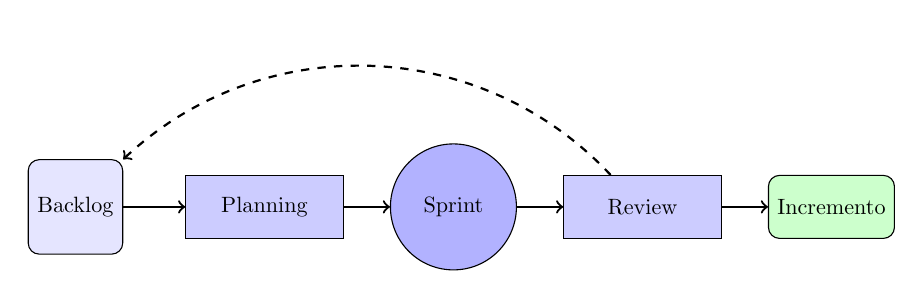
\begin{tikzpicture}[node distance=2.5cm, auto, scale=0.8, transform shape]
    \node (backlog) [draw, rectangle, rounded corners, minimum height=1.5cm, minimum width=1.5cm, fill=blue!10] {Backlog};
    \node (sprintplan) [draw, rectangle, minimum width=2.5cm, minimum height=1cm, fill=blue!20, right of=backlog, node distance=3cm] {Planning};
    \node (sprint) [draw, circle, minimum size=2cm, fill=blue!30, right of=sprintplan, node distance=3cm] {Sprint};
    \node (review) [draw, rectangle, minimum width=2.5cm, minimum height=1cm, fill=blue!20, right of=sprint, node distance=3cm] {Review};
    \node (inc) [draw, rectangle, rounded corners, minimum width=2cm, minimum height=1cm, fill=green!20, right of=review, node distance=3cm] {Incremento};

    \draw[->, thick] (backlog) -- (sprintplan);
    \draw[->, thick] (sprintplan) -- (sprint);
    \draw[->, thick] (sprint) -- (review);
    \draw[->, thick] (review) -- (inc);
    \draw[->, thick, dashed] (review) to[bend right=45] (backlog);
\end{tikzpicture}
\captionof{figure}{Ciclo de Vida de Scrum}
\end{center}
\vspace{0.5cm}
\newpage
\subsubsection{Kanban}
\textbf{Enfoque:} Está basado en los principios Lean y se centra en hacer visible el flujo de trabajo y en entregar de forma continua. En vez de usar Sprints de duración fija, regula el ritmo limitando la cantidad de tareas que pueden estar en curso al mismo tiempo, lo que se conoce como límite de trabajo en progreso o WIP (Work in Progress) \citep{anderson2010kanban}.

\textbf{Fases o Prácticas Principales:}
\begin{enumerate}
    \item Visualización del flujo: Se dibuja el proceso en columnas (por ejemplo, Por Hacer, En Desarrollo, Pruebas y Hecho).
    \item Límites de WIP: Se fija un máximo de tareas por columna.
    \item Control del flujo: Se revisa el avance para resolver rápido los bloqueos.
    \item Mejora continua: El proceso se va ajustando con el tiempo.
\end{enumerate}

\textbf{Representación Gráfica:}
\vspace{0.5cm}
\begin{center}
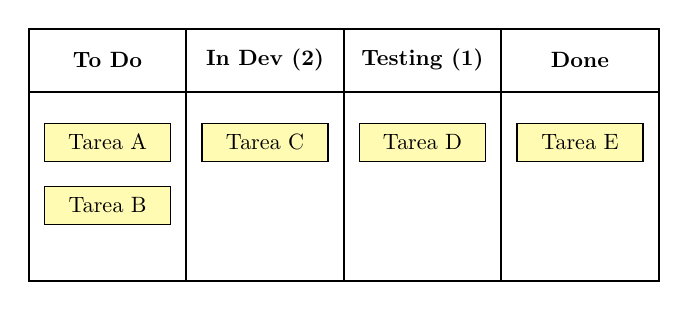
\begin{tikzpicture}[scale=0.8, transform shape]
    % Tablero
    \draw[thick] (0,0) rectangle (10,4);
    \draw[thick] (2.5,0) -- (2.5,4);
    \draw[thick] (5,0) -- (5,4);
    \draw[thick] (7.5,0) -- (7.5,4);

    % Cabeceras
    \node at (1.25, 3.5) {\textbf{To Do}};
    \node at (3.75, 3.5) {\textbf{In Dev (2)}};
    \node at (6.25, 3.5) {\textbf{Testing (1)}};
    \node at (8.75, 3.5) {\textbf{Done}};
    \draw[thick] (0,3) -- (10,3);

    % Tarjetas
    \node[draw, fill=yellow!30, minimum width=2cm, minimum height=0.6cm] at (1.25, 2.2) {Tarea A};
    \node[draw, fill=yellow!30, minimum width=2cm, minimum height=0.6cm] at (1.25, 1.2) {Tarea B};
    \node[draw, fill=yellow!30, minimum width=2cm, minimum height=0.6cm] at (3.75, 2.2) {Tarea C};
    \node[draw, fill=yellow!30, minimum width=2cm, minimum height=0.6cm] at (6.25, 2.2) {Tarea D};
    \node[draw, fill=yellow!30, minimum width=2cm, minimum height=0.6cm] at (8.75, 2.2) {Tarea E};
\end{tikzpicture}
\captionof{figure}{Tablero Kanban Básico}
\end{center}
\vspace{0.5cm}
\newpage
\subsubsection{Prototipo Evolutivo}
\textbf{Enfoque:} Es un modelo en el que se construye rápidamente una primera versión funcional del sistema, que se muestra al usuario y se va mejorando en versiones sucesivas hasta convertirse en el producto final. A diferencia del prototipo desechable, que solo sirve para aclarar requisitos y después se descarta, en el prototipo evolutivo el código no se bota, sino que cada versión parte de la anterior. Es útil cuando los requisitos no están del todo claros al inicio y se necesita ver algo funcionando para definirlos mejor \citep{sommerville2015, pressman2010}.

\textbf{Fases o Etapas:}
\begin{enumerate}
    \item Comunicación: Se identifican con los usuarios los requisitos generales que ya se conocen.
    \item Diseño rápido: Se diseña de forma simple lo que el usuario va a ver, como las pantallas y el flujo principal.
    \item Construcción del prototipo: Se programa una versión funcional con las partes más importantes.
    \item Evaluación: El usuario prueba el prototipo y entrega sus comentarios.
    \item Refinamiento: Con esos comentarios se mejora el prototipo y se vuelve a evaluar, hasta llegar al producto final.
\end{enumerate}

\textbf{Representación Gráfica:}
\vspace{0.5cm}
\begin{center}
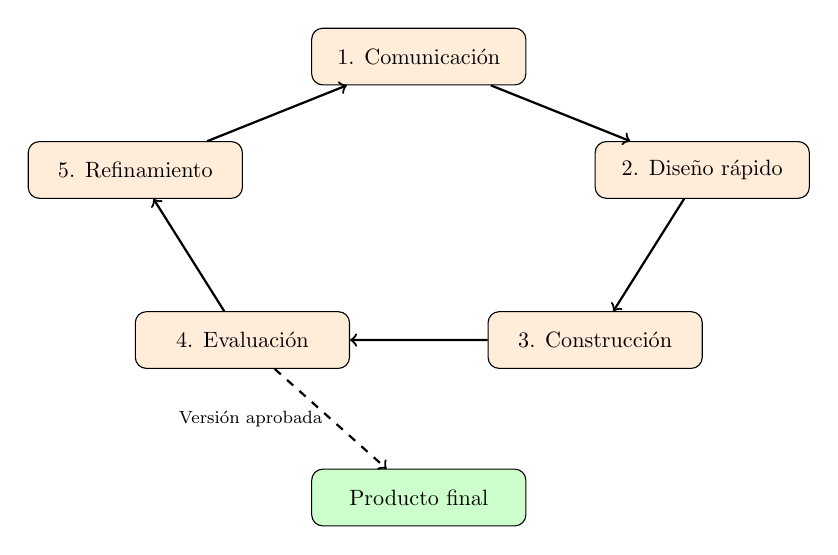
\begin{tikzpicture}[scale=0.8, transform shape,
    box/.style={draw, rectangle, rounded corners, minimum width=3.4cm, minimum height=0.9cm, fill=orange!15, text centered}]
    \node (com) [box] at (0,3) {1. Comunicación};
    \node (dis) [box] at (4.5,1.2) {2. Diseño rápido};
    \node (con) [box] at (2.8,-1.5) {3. Construcción};
    \node (eva) [box] at (-2.8,-1.5) {4. Evaluación};
    \node (ref) [box] at (-4.5,1.2) {5. Refinamiento};
    \node (fin) [draw, rectangle, rounded corners, minimum width=3.4cm, minimum height=0.9cm, fill=green!20] at (0,-4) {Producto final};

    \draw[->, thick] (com) -- (dis);
    \draw[->, thick] (dis) -- (con);
    \draw[->, thick] (con) -- (eva);
    \draw[->, thick] (eva) -- (ref);
    \draw[->, thick] (ref) -- (com);
    \draw[->, thick, dashed] (eva) -- node[left, font=\footnotesize] {Versión aprobada} (fin);
\end{tikzpicture}
\captionof{figure}{Ciclo del Prototipo Evolutivo}
\end{center}
\vspace{0.5cm}
\newpage
\subsection{Evaluación de Alternativas}
Para elegir la metodología más adecuada, los tres enfoques se evaluaron según los siguientes criterios:

\begin{itemize}
    \item \textbf{Aplicabilidad:} Qué tan bien se adapta a proyectos con mucha innovación, integración de APIs y modelos de cálculo.
    \item \textbf{Eficiencia:} Qué tan rápido permite tener entregables y versiones funcionales.
    \item \textbf{Costo y riesgos:} Qué tan fácil es reducir riesgos o cambiar de rumbo sin un gran costo.
    \item \textbf{Calidad:} Qué tanto favorece la validación constante, las pruebas y la retroalimentación.
    \item \textbf{Adaptabilidad:} Qué tan flexible es para incorporar cambios en los requisitos en etapas avanzadas.
    \item \textbf{Ajuste a un solo desarrollador:} Qué tan bien funciona cuando todo el trabajo lo hace una sola persona.
    \item \textbf{Carga de documentación:} Cuánto trabajo exige documentar el proceso, como reuniones, tableros y registros de avance.
    \item \textbf{Ajuste al plazo del MVP:} Qué tanto ayuda a llegar a un producto mínimo viable antes de diciembre de 2026.
\end{itemize}
\newpage
\subsection{Cuadro Comparativo}
\begin{table}[h!]
    \centering
    \renewcommand{\arraystretch}{1.4}
    \begin{tabular}{|m{2.9cm}|m{3.8cm}|m{3.8cm}|m{3.8cm}|}
        \hline
        \rowcolor[HTML]{EFEFEF}
        \textbf{Criterio} & \textbf{Scrum (Ágil)} & \textbf{Kanban (Lean/Ágil)} & \textbf{Prototipo evolutivo} \\ \hline
        \textbf{Aplicabilidad} & Alta. Permite probar las integraciones en ciclos cortos. & Alta. El flujo continuo permite incorporar cambios día a día. & Alta. Sirve cuando los requisitos no están claros, como en el cálculo de la fatiga cruzada. \\ \hline
        \textbf{Eficiencia} & Alta. Entrega partes funcionales al final de cada Sprint. & Media-Alta. Entrega continua, enfocada en evitar atascos. & Alta. Desde temprano hay una versión que se puede usar y probar. \\ \hline
        \textbf{Costo y riesgos} & Bajo riesgo. Los errores se detectan en las primeras iteraciones. & Bajo riesgo. Los bloqueos se ven de inmediato. & Riesgo medio. Detecta temprano errores en los requisitos, pero el código puede crecer desordenado si no se revisa. \\ \hline
        \textbf{Calidad} & Validación constante en cada Sprint Review. & Alta, gracias al límite de trabajo en curso (WIP). & Retroalimentación constante del usuario, aunque la estructura interna puede deteriorarse. \\ \hline
        \textbf{Adaptabilidad} & Alta. Los requerimientos se pueden ajustar entre Sprints. & Muy alta. Las prioridades cambian según se necesite. & Muy alta. Cada nueva versión incorpora los cambios. \\ \hline
        \textbf{Un solo desarrollador} & Baja. Sus roles y reuniones están pensados para equipos. & Alta. Funciona igual con una sola persona. & Alta. No exige roles ni reuniones fijas. \\ \hline
        \textbf{Carga de documentación} & Alta. Hay que registrar el Product Backlog, la planificación, la revisión y la retrospectiva de cada Sprint. & Media-Alta. Hay que mantener al día el tablero, los límites de trabajo y el registro del flujo. & Baja. Se documenta cada versión del prototipo y el resultado de su evaluación. \\ \hline
        \textbf{Ajuste al plazo del MVP} & Media. Ordena el avance, pero sus reuniones restan tiempo de desarrollo. & Media. Ayuda a terminar tareas, pero no define cuándo se entrega una versión. & Alta. Cada versión acerca la aplicación al MVP final. \\ \hline
    \end{tabular}
    \caption{Cuadro comparativo de alternativas metodológicas.}
    \label{tab:comparativa_metodologias}
\end{table}
\newpage
\subsection{Justificación Metodología Seleccionada}

Después de evaluar las alternativas, se eligió el \textbf{modelo de prototipo evolutivo} como metodología de desarrollo del proyecto. Scrum y Kanban fueron analizadas porque son metodologías muy usadas y con buenos resultados, pero se descartaron por las siguientes razones:
\begin{itemize}
    \item \textbf{Scrum:} Está pensado para equipos, con roles y reuniones que no tienen mucho sentido cuando el desarrollo lo hace una sola persona. Además, exige documentar todo el proceso (Product Backlog, planificación, revisión y retrospectiva de cada Sprint), lo que le quita tiempo al desarrollo.
    \item \textbf{Kanban:} Ordena muy bien el trabajo diario, pero también requiere mantener al día el tablero y el registro del flujo. Además, por sí solo no define en qué momento se entrega una versión funcional para evaluarla.
\end{itemize}

El prototipo evolutivo, en cambio, se ajusta mejor a este proyecto por cuatro motivos:
\begin{itemize}
    \item \textbf{Los requisitos se aclaran con el uso:} El cálculo de la fatiga cruzada y las sugerencias de nutrición necesitan probarse para saber si funcionan bien. Con un prototipo funcional se pueden ajustar a partir de lo que se observa en cada evaluación.
    \item \textbf{Menos documentación de proceso:} Solo se documenta cada versión y su evaluación, lo que es más realista para una sola persona que además debe cumplir con los plazos académicos.
    \item \textbf{Lleva directo al MVP:} El código no se bota. Cada versión parte de la anterior, por lo que la última versión del prototipo es el producto mínimo viable que plantea el objetivo general.
    \item \textbf{Permite probar temprano si la aplicación es fácil de usar:} Uno de los problemas identificados en el Capítulo 2 es lo engorroso que resulta usar las aplicaciones actuales. Con un prototipo se puede comprobar desde el inicio si la aplicación es simple de usar.
\end{itemize}

Para controlar el principal riesgo de este modelo, que es que el código crezca de forma desordenada, al final de cada versión se reservará tiempo para ordenar el código, y el backend se organizará en módulos independientes desde el comienzo.
\newpage
\subsection{Diseño del Plan Metodológico del Proyecto}

El desarrollo se organiza en versiones sucesivas del prototipo, de 2 a 3 semanas cada una. Cada versión pasa por las cinco fases del modelo:

\begin{enumerate}
    \item \textbf{Fase 1: Comunicación:}
    Se definen los requisitos que se abordarán en la versión, a partir de los requerimientos del sistema y de los resultados de la versión anterior.

    \item \textbf{Fase 2: Diseño rápido:}
    Se diseñan las pantallas y el flujo de las funciones nuevas, junto con los cambios necesarios en la base de datos y en los servicios del backend.

    \item \textbf{Fase 3: Construcción del prototipo:}
    Se programan las funciones de la versión sobre el prototipo existente. Para no dispersar el trabajo, se aborda un componente pesado a la vez, por ejemplo el módulo de cardio o el procesamiento de lenguaje natural.

    \item \textbf{Fase 4: Evaluación:}
    Se hacen pruebas técnicas, por ejemplo simulando datos de un wearable o verificando que las metas nutricionales se ajusten bien al gasto registrado. También se prueba el prototipo con usuarios para recoger sus comentarios.

    \item \textbf{Fase 5: Refinamiento:}
    Con los resultados de la evaluación se corrigen errores, se ordena el código y se definen los ajustes para la siguiente versión. Cuando una versión cumple con todos los requerimientos del MVP, se cierra el ciclo.
\end{enumerate}

Las versiones del prototipo se planifican de la siguiente forma:

\begin{center}
    \renewcommand{\arraystretch}{1.4}
    \begin{tabular}{|>{\raggedright\arraybackslash}m{3.0cm}|m{11.9cm}|}
        \hline
        \rowcolor[HTML]{EFEFEF}
        \textbf{Versión} & \textbf{Contenido principal} \\ \hline
        \textbf{Versión 1} & Creación de la cuenta con los términos de uso y el aviso legal, cuestionario inicial del perfil del usuario y registro manual de entrenamientos de fuerza y de comidas, con los catálogos de ejercicios y alimentos, incluida la lectura de códigos de barras. \\ \hline
        \textbf{Versión 2} & Registro de entrenamientos de resistencia con el GPS del teléfono y lectura automática desde Health Connect y Apple Health. \\ \hline
        \textbf{Versión 3} & Registro asistido por inteligencia artificial (lenguaje natural y fotos de comida) y carga de archivos \texttt{.fit}. \\ \hline
        \textbf{Versión 4} & Cruce de datos: cálculo de fatiga, alertas, metas de alimentación según el entrenamiento, línea de tiempo del progreso y plan semanal sugerido según el perfil. \\ \hline
        \rowcolor[HTML]{E8F5E9}
        \textbf{Versión 5 (MVP)} & Red social básica (seguir usuarios, publicar sesiones, rutas y comidas con fotos en el perfil y agregarlas a los propios módulos), panel de administración, control de datos personales y suscripción al plan premium. Con esta versión se completa el MVP. \\ \hline
        \textbf{Después del MVP} & Récords de tramo, récords de fuerza comparados, retos entre seguidores y videos en las publicaciones. \\ \hline
    \end{tabular}
    \captionof{table}{Planificación de las versiones del prototipo evolutivo.}
    \label{tab:versiones_prototipo}
\end{center}

Hay que distinguir entre el prototipo de demostración y el MVP. El prototipo que se usa hoy en las pruebas deja fuera la subida de fotos, para ahorrar costos de almacenamiento mientras se desarrolla. El MVP, en cambio, sí permite publicar fotos, porque es la primera versión que llegará a usuarios reales y lo visual es uno de los mayores atractivos de una red social. Por eso las fotos se suman en la versión 5, junto con el resto de la red social.

\vspace{0.5cm}
\begin{center}
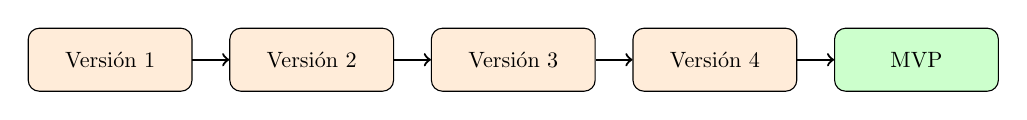
\begin{tikzpicture}[node distance=3.2cm, scale=0.8, transform shape,
    box/.style={draw, rectangle, rounded corners, minimum width=2.6cm, minimum height=1cm, fill=orange!15, text centered}]
    \node (v1) [box] {Versión 1};
    \node (v2) [box, right of=v1] {Versión 2};
    \node (v3) [box, right of=v2] {Versión 3};
    \node (v4) [box, right of=v3] {Versión 4};
    \node (v5) [box, right of=v4, fill=green!20] {MVP};
    \draw[->, thick] (v1) -- (v2);
    \draw[->, thick] (v2) -- (v3);
    \draw[->, thick] (v3) -- (v4);
    \draw[->, thick] (v4) -- (v5);
\end{tikzpicture}
\captionof{figure}{Evolución del prototipo hasta el MVP}
\end{center}

\subsection{Comentarios Generales del Capítulo}

En resumen, definir la metodología permite ordenar el trabajo y reducir la incertidumbre propia de este proyecto. Se analizaron Scrum, Kanban y el prototipo evolutivo, y se eligió este último. Scrum y Kanban se descartaron porque exigen documentar y mantener todo el proceso, algo poco práctico para una sola persona con un plazo acotado. El prototipo evolutivo, en cambio, permite tener una versión funcional desde temprano, ajustar los requisitos con lo que se aprende en cada evaluación y llegar al MVP con la última versión. Con esta base, en el siguiente capítulo se presentan las alternativas de solución y los estudios de factibilidad técnica, económica y operativa.
\newpage
